\documentclass[12pt,a4paper]{article}
\usepackage[utf8]{inputenc}
\usepackage[T1]{fontenc}
\usepackage[brazil]{babel}
\usepackage[margin=2.5cm]{geometry}
\usepackage{booktabs}
\usepackage{amsmath,amssymb}
\usepackage{caption}
\usepackage{graphicx}
\usepackage{setspace}
\usepackage{indentfirst}
\usepackage{fancyhdr}
\usepackage[hidelinks]{hyperref}
\graphicspath{{docs/}}

\captionsetup{font=small,labelsep=colon}
\onehalfspacing

\pagestyle{fancy}
\fancyhf{}
\fancyhead[L]{\footnotesize Determinantes e previsibilidade dos pesos de ações em fundos}
\fancyhead[R]{\footnotesize J. P. Zangrandi}
\fancyfoot[C]{\thepage}
\renewcommand{\headrulewidth}{0.4pt}

\begin{document}

%==================== CAPA ====================
\thispagestyle{empty}
\begin{center}
{\large FUNDAÇÃO GETÚLIO VARGAS}\\[2pt]
{\large ESCOLA DE ECONOMIA DE SÃO PAULO}\\[16pt]
{\normalsize Graduação em Economia}

\vspace{3.5cm}

{\large João Paulo Zangrandi}

\vspace{2.5cm}

{\Large Determinantes e previsibilidade dos pesos de ações em fundos de investimento:}\\[12pt]
{\large uma aplicação de fator dinâmico ao caso de VALE3 nas carteiras do Itaú entre 2016 e 2021}

\vspace{2.5cm}

\begin{flushright}
\begin{minipage}{0.62\textwidth}
\small\setstretch{1.15}
Monografia I apresentada à Escola de Economia de São Paulo da Fundação Getúlio
Vargas como requisito da disciplina Monografia I.
\\[10pt]
Orientador: Prof.\ Maurício Ferraresi Junior.
\end{minipage}
\end{flushright}

\vfill

{\normalsize São Paulo}\\
{\normalsize 2026}
\end{center}

\newpage

%==================== RESUMO / ABSTRACT ====================
\thispagestyle{fancy}
\begin{center}{\large Resumo}\end{center}
\noindent
Este trabalho estuda, de forma empírica, os determinantes e a previsibilidade do peso da
ação VALE3 nas carteiras dos fundos da gestora Itaú, no painel mensal de 2016 a 2021.
A abordagem segue a lógica de um sistema de demanda: para cada mês, o peso da ação em
cada fundo é regredido por mínimos quadrados sobre um conjunto de características de fundo
e de ação, e os coeficientes dessa regressão transversal são interpretados como um fator
latente que resume como as posições dependem dessas características. Ao deixar esse fator
variar ao longo do tempo, obtém-se um modelo de fator dinâmico, que serve tanto para
explicar a seção transversal das posições quanto para prever o peso em meses seguintes.
Os resultados indicam que o peso é bem explicado pelo tamanho do fundo, pelo número de
cotistas e pela classificação do fundo como fundo de investimento em cotas, com sinais
estáveis ao longo dos 72 meses, e que a decisão de ter ou não a ação carrega sinais
opostos aos da decisão de quanto carregar, um padrão compatível com diversificação. Para
previsão, contudo, nenhum dos modelos estruturais testados, incluindo efeito fixo de fundo
e filtro de Kalman, supera a previsão ingênua de repetir o último peso observado, mesmo sob
a defasagem trimestral de divulgação das carteiras. O peso comporta-se, no nível do fundo,
de forma muito persistente, próxima de um passeio aleatório. O trabalho encerra com a
especificação do passo seguinte, um modelo de ajuste parcial da carteira a ser estimado na
continuação.

\smallskip
\noindent Palavras-chave: sistema de demanda; fundos de investimento; pesos de carteira;
fator dinâmico; previsão; mercado acionário brasileiro.

\bigskip
\begin{center}{\large Abstract}\end{center}
\noindent
This paper empirically studies the determinants and the predictability of the portfolio
weight of the stock VALE3 across mutual funds managed by Itaú, on a monthly panel from 2016
to 2021. The approach follows the logic of a demand system: for each month, the stock weight
in each fund is regressed by ordinary least squares on a set of fund and stock
characteristics, and the coefficients of this cross-sectional regression are read as a latent
factor that summarizes how positions depend on these characteristics. Letting this factor
vary over time yields a dynamic factor model, useful both to explain the cross-section of
positions and to forecast the weight in subsequent months. The results show that the weight
is well explained by fund size, the number of shareholders, and the fund-of-funds
classification, with stable signs across the 72 months, and that the decision to hold the
stock carries signs opposite to the decision of how much to hold, a pattern consistent with
diversification. For forecasting, however, none of the structural models tested, including a
fund fixed effect and a Kalman filter, beats the naïve forecast of repeating the last
observed weight, even under the quarterly disclosure lag of portfolios. The weight behaves,
at the fund level, very persistently, close to a random walk. The paper closes with the
specification of the next step, a partial portfolio adjustment model to be estimated in the
sequel.

\smallskip
\noindent Keywords: demand system; mutual funds; portfolio weights; dynamic factor;
forecasting; Brazilian equity market.

\newpage
\thispagestyle{fancy}
\tableofcontents
\newpage

%==================== 1. INTRODUÇÃO ====================
\section{Introdução}

A composição das carteiras dos fundos de investimento é uma das informações mais ricas e
ao mesmo tempo menos exploradas do mercado de capitais brasileiro. Quando um fundo decide
quanto de cada ação carregar, ele revela, ainda que parcialmente, a sua demanda por aquele
papel. Olhar para todos os fundos de uma mesma gestora ao mesmo tempo equivale, então, a
observar um grande conjunto de decisões de demanda tomadas sob informações e incentivos
parecidos, o que torna possível investigar de forma organizada duas perguntas. A primeira
é quais características de um fundo explicam o peso que ele atribui a uma ação. A segunda é
se esse peso pode ser previsto de um mês para o outro.

Para tornar o problema tratável, este trabalho concentra-se em um caso concreto. Estuda-se
o peso da ação VALE3, considerada apenas como posição direta, nas carteiras dos fundos das
três gestoras do grupo Itaú, a saber, Itaú Asset Management, Itaú DTVM e Itaú Unibanco, no
período de 2016 a 2021. A escolha do peso como variável de interesse, em vez do valor
financeiro ou do número de ações, é deliberada. O peso é limitado entre zero e um, o que o
torna mais simples de modelar; é comparável entre fundos de tamanhos muito distintos; e
corresponde diretamente à noção de demanda relativa que organiza os modelos de demanda por
ativos.

O arcabouço teórico de referência é o sistema de demanda de Koijen e Yogo (2019), que
propõem tratar os preços dos ativos como resultado das demandas de investidores que escolhem
suas carteiras em função das características dos ativos. A principal vantagem dessa
abordagem é reduzir um problema de dimensão muito alta, com milhares de ativos e
investidores, a um número pequeno de parâmetros associados às características. O presente
trabalho situa-se no lado das quantidades desse programa: em vez de estimar como a demanda
reage a preços, estima-se como o peso de uma ação reage às características dos fundos que a
carregam. Em linha próxima, Gabaix e Koijen (2021) argumentam que os mercados são pouco
elásticos, de modo que fluxos de demanda têm efeito expressivo sobre preços, o que reforça
o interesse em medir diretamente a demanda dos investidores institucionais, justamente o que
as carteiras dos fundos permitem observar.

Do ponto de vista do método, a estratégia adotada é estimar os coeficientes da regressão
mês a mês e, em seguida, resumir a média e a variação desses coeficientes ao longo do tempo,
procedimento consagrado por Fama e MacBeth (1973) na literatura empírica de apreçamento de
ativos. Quando a sequência de coeficientes passa a ser tratada como uma série temporal, e
quando se procura separar o sinal persistente do ruído de estimação de cada mês, recorre-se
à ideia de modelos de espaço de estados e ao filtro de Kalman, apresentados de forma
didática por Harvey (1989). Como uma das características empregadas é o fluxo líquido dos
fundos, é pertinente a literatura que liga fluxos à negociação: Coval e Stafford (2007)
mostram que fundos pressionados por resgates são forçados a vender e que entradas levam a
compras, com efeito sobre preços, e Lou (2012) relaciona fluxos à previsibilidade de
retornos. O fluxo é incluído precisamente para testar se ele ajuda a antecipar a variação do
peso da ação na carteira.

A pergunta de previsão é avaliada contra uma referência exigente, a previsão ingênua que
apenas repete o último valor observado, seguindo a disciplina usual dessa literatura,
segundo a qual um modelo só interessa se conseguir superar essa regra simples. No caso
brasileiro, a evidência sobre demanda por ativos a partir de carteiras de fundos é escassa,
o que motiva organizar, de forma reprodutível e a partir das bases públicas da Comissão de
Valores Mobiliários, um painel de pesos de carteira e um conjunto de exercícios de
explicação e de previsão.

O resultado central que emerge tem dois lados. Para explicar o peso, as características
funcionam bem: fundos maiores carregam menos VALE3 em peso, fundos com mais cotistas carregam
mais, e os fundos de cotas têm posição direta menor, com sinais que se repetem em todos os
meses da amostra. Para prever, no entanto, nenhum dos modelos estruturais testados supera a
regra simples de repetir o último peso. Em outras palavras, no nível de cada fundo o peso é
muito persistente e comporta-se quase como um passeio aleatório. Esse contraste, entre um bom
poder de explicação e um fraco poder de previsão de curto prazo, é o que se considera o
achado principal desta entrega.

O restante do texto está organizado da seguinte forma. A Seção 2 descreve os dados e seu
tratamento. A Seção 3 detalha a metodologia, incluindo a especificação do modelo de ajuste
parcial que será estimado na continuação do trabalho. A Seção 4 apresenta e interpreta os
resultados. A Seção 5 conclui e aponta a agenda futura.

%==================== 2. DADOS ====================
\section{Dados}

A base empírica reúne duas fontes principais da Comissão de Valores Mobiliários e uma fonte
de mercado para o preço da ação. A primeira fonte é a composição consolidada das carteiras
dos fundos, de frequência mensal, da qual se extrai o peso de VALE3 em cada fundo, sempre
tomado como posição direta no ativo identificado como VALE ON. A segunda é a série histórica
diária dos fundos, da qual se obtêm o patrimônio líquido, o número de cotistas e a informação
de o fundo ser ou não um fundo de investimento em cotas. A captação líquida, isto é, a
captação menos os resgates, é obtida do Informe Diário da mesma Comissão, que é a base de
origem da série histórica e a única que registra os resgates. O preço e o beta de VALE3 são
calculados a partir de cotações de mercado.

O tratamento dos dados privilegia a consistência e a ausência de informação espúria. O nome
da gestora é padronizado, removendo acentuação, caixa e sufixos, de modo a reunir
corretamente as três variações do grupo Itaú. Linhas exatamente duplicadas da base de
composição, que a Comissão ocasionalmente repete, são colapsadas. Pesos negativos, que
aparecem apenas como resíduos contábeis de magnitude desprezível, são descartados, pois não
têm interpretação como participação na carteira. Após montar o painel, verifica-se que não
há par de fundo e mês repetido. Os fundos exclusivos são retirados por meio de um critério
simples, mantendo-se apenas as observações com mais de três cotistas, uma vez que fundos com
um ou dois cotistas refletem decisões de um único investidor e não a demanda difusa que se
quer estudar. O casamento entre a base diária e a base mensal é feito pelo dia exato da
competência, sem perda de observações.

Dois cuidados de validação merecem registro. Primeiro, a captação líquida obtida do Informe
Diário foi confrontada com a informação correspondente da série histórica, e a coincidência
é quase perfeita, com mais de noventa e nove por cento dos pares de fundo e mês batendo ao
centavo; as poucas divergências decorrem de diferenças entre as duas séries da própria
Comissão, e não de erro de processamento. Segundo, o preço de VALE3 foi conferido contra o
fechamento oficial da bolsa nas datas de referência utilizadas, sem diferença relevante. O
beta é calculado como a razão entre a covariância dos retornos da ação e do Ibovespa e a
variância dos retornos do índice, em janela móvel de duzentos e cinquenta e dois pregões.

Aplicados esses critérios, o painel cobre os 72 meses entre 2016 e 2021 e abrange as três
gestoras do grupo Itaú. O painel completo de fundos que detêm a ação reúne 26.123 observações
de fundo por mês, distribuídas em 623 fundos. A amostra que entra nas regressões de
explicação, restrita aos fundos com mais de três cotistas e com fluxo disponível, contém
11.413 observações de fundo por mês, provenientes de 307 fundos, das quais cerca de três
quartos correspondem a fundos de cotas. A Tabela~\ref{tab:desc} resume as variáveis nessa
amostra.

\begin{table}[h]\centering\small
\caption{Estatísticas descritivas da amostra de regressão (11.413 observações de fundo por mês, 2016--2021).}
\label{tab:desc}
\begin{tabular}{@{}lrrrrr@{}}
\toprule
Variável & Média & Desvio-padrão & Mediana & Mínimo & Máximo \\
\midrule
Peso de VALE3 (\%)            & $2{,}87$ & $3{,}52$ & $1{,}22$ & $0{,}00$ & $23{,}55$ \\
Patrimônio líquido (R\$ mi)   & $399$    & $1.079$  & $68{,}3$ & $0{,}04$ & $17.866$ \\
Número de cotistas            & $10.202$ & $72.039$ & $105$    & $4$      & $696.013$ \\
Captação líquida (R\$ mi)     & $5{,}7$  & $74{,}1$ & $0{,}0$  & $-1.522$ & $1.636$ \\
Preço de VALE3 (R\$)          & $54{,}6$ & $27{,}2$ & $50{,}9$ & $9{,}94$ & $114{,}1$ \\
Beta de VALE3                 & $1{,}04$ & $0{,}30$ & $0{,}97$ & $0{,}68$ & $1{,}73$ \\
\bottomrule
\end{tabular}
\caption*{\footnotesize Fonte: Comissão de Valores Mobiliários e cotações de mercado; elaboração própria.}
\end{table}

O patrimônio líquido e o número de cotistas são fortemente assimétricos, com média muito
acima da mediana, razão pela qual se adota o logaritmo dessas variáveis nas regressões. Vale
notar ainda que o preço e o beta de VALE3 são bastante correlacionados de forma negativa no
período, com correlação em torno de menos zero vírgula setenta e um, refletindo a recuperação
da ação entre 2016 e 2021, em que o preço subiu enquanto a volatilidade relativa ao mercado
recuou.

%==================== 3. METODOLOGIA ====================
\section{Metodologia}

\subsection{Especificação de demanda}

Sejam os fundos de uma gestora, indexados por $i$, e uma ação, indexada por $n$. Para cada
fundo $i$ e cada mês $t$, a variável de interesse é o peso $w_{i,t}$ da ação na carteira,
limitado ao intervalo entre zero e um. A leitura adotada é a de que o peso observado é um
peso desejado mais um componente aleatório,
\begin{equation}
w_{i,t} = w^{*}_{i,t} + \varepsilon_{i,t}, \qquad w^{*}_{i,t} = x_{i,t}'\,\theta_{n,t},
\label{eq:target}
\end{equation}
em que $x_{i,t}$ é o vetor de características do fundo e $\theta_{n,t}$ é um vetor de fatores
latentes associados à ação, que mede o quanto cada característica importa para a posição
naquele papel. As características desempenham, nessa leitura, o papel de descrever o perfil de
cada fundo, e os fatores latentes resumem como a ação é demandada em função desse perfil.

\subsection{Primeiro passo: a regressão transversal e o fator latente}

O primeiro passo estima os fatores latentes. Empilhando os fundos vivos em cada mês $t$,
escreve-se $w_t = X_t\,\theta_{n,t} + \varepsilon_t$ e estima-se por mínimos quadrados,
\begin{equation}
\widehat{\theta}_{n,t} = (X_t'X_t)^{-1} X_t'\,w_t,
\label{eq:ols}
\end{equation}
com as características padronizadas, isto é, com média zero e variância um, para que sejam
comparáveis entre si. Na prática, a regressão estimada em cada mês é
\begin{equation}
w_{i,t} = \alpha_t + \beta^{1}_t \ln(\text{PL}_{i,t}) + \beta^{2}_t \ln(\text{Cot}_{i,t})
        + \beta^{3}_t \text{FIC}_i + \beta^{4}_t \Big(\tfrac{\text{Fluxo}}{\text{PL}}\Big)_{i,t}
        + \varepsilon_{i,t},
\label{eq:cs}
\end{equation}
em que PL é o patrimônio líquido, Cot é o número de cotistas, FIC indica se o fundo é um
fundo de investimento em cotas e Fluxo é a captação líquida do mês. Estimada nos 72 meses,
essa regressão gera 72 vetores de coeficientes, resumidos pela média no tempo e por um erro
padrão calculado a partir da variação dos coeficientes entre os meses, no espírito de Fama e
MacBeth (1973). O preço e o beta da ação são constantes dentro de um mesmo mês e, por isso,
não entram na regressão mês a mês; eles são incluídos em uma versão com todos os meses
empilhados, na qual passam a ser identificados pela variação entre meses. Como o peso é
limitado entre zero e um, a forma mais adequada seria não linear, com uma função logística, o
que se utiliza adiante para estudar a decisão de ter ou não a ação.

\subsection{Segundo passo: dinâmica do fator e previsão}

O segundo passo dá dinâmica ao fator e o utiliza para prever. Cada coeficiente
$\theta_{k,t}$ é tratado como uma série temporal, modelada como passeio aleatório, como um
processo autorregressivo de primeira ordem ou por um modelo de espaço de estados estimado
pelo filtro de Kalman. A previsão do peso aplica o vetor de coeficientes previsto às
características do fundo, $\widehat{w}_{i,t} = \widehat{\theta}_t'\,x_{i,t}$, e é comparada à
previsão ingênua que repete o peso do mês anterior, $\widehat{w}_{i,t}=w_{i,t-1}$. A diferença
entre o realizado e o previsto forma o conjunto de erros $e_{i,t}=w_{i,t}-\widehat{w}_{i,t}$,
cujas propriedades são analisadas, em particular se a média é próxima de zero e se a série é
estacionária. A avaliação é feita fora da amostra, com janela de estimação expandida, para os
horizontes de um e de três meses. O horizonte de três meses tem motivação econômica: como as
carteiras só são divulgadas com cerca de noventa dias de defasagem, conhecer o peso de hoje
equivale, na prática, a prever o peso de três meses à frente usando apenas a informação
disponível até hoje.

Um cuidado central é não utilizar informação do futuro ao prever. Cada característica é
medida em um momento bem definido em relação ao peso do mês $t$. O peso e as características de
fundo são medidos ao final do mês $t$; o fluxo é somado ao longo do mês $t$; e o preço e o
beta da ação têm dois usos distintos. Para explicar o peso, emprega-se a média do mês $t$, que
representa melhor o que o gestor observou ao longo do mês ao dimensionar a posição. Para
prever, emprega-se o valor do final do mês anterior, conhecido antes de $t$ e, portanto, livre
de informação futura.

\subsection{A decisão de ter ou não a ação}

As regressões anteriores tratam do peso condicional a o fundo deter a ação, isto é, da
chamada margem intensiva. A decisão de ter ou não a ação, a margem extensiva, é estudada à
parte, em um painel que inclui também os fundos de ações que não detêm VALE3, com peso igual
a zero. Para essa decisão, estima-se uma regressão logística da probabilidade de o fundo ter
a ação sobre o logaritmo do patrimônio, o logaritmo do número de cotistas e a classificação
de fundo de cotas, o que permite comparar quais características explicam ter a ação e quais
explicam quanto dela carregar.

\subsection{Extensão dinâmica: o modelo de ajuste parcial}

A continuação natural do trabalho, a ser estimada na sequência, parte da mesma especificação
de demanda e a torna mais completa em dois pontos. Primeiro, escreve-se o peso desejado como
uma função logística do produto entre as características do fundo e os fatores latentes da
ação, $w_{i,n} = g(x_i'\,\theta_n) + \varepsilon_{i,n}$, mantendo a estimação do vetor de
fatores mês a mês, como já feito nesta entrega. Segundo, e principalmente, modela-se de forma
explícita como o fundo ajusta a posição de um mês para o outro.

A hipótese é a de que o fundo não salta de uma só vez para o peso desejado, mas se move
parcialmente em sua direção, a uma velocidade de ajuste $\lambda_n$ situada entre zero e um,
\begin{equation}
w_{i,t+1} = (1-\lambda_n)\,w_{i,t} + \lambda_n\,w^{*}_{i,t} + u_{i,t+1}.
\label{eq:pa1}
\end{equation}
Reescrevendo essa relação em termos da variação do peso, e definindo $\varepsilon_{i,t}=
w^{*}_{i,t}-w_{i,t}$ como a distância entre o peso desejado e o peso atual, obtém-se uma forma
simples de estimar,
\begin{equation}
w_{i,t+1}-w_{i,t} = \lambda_n\,\varepsilon_{i,t} + u_{i,t+1}.
\label{eq:pa2}
\end{equation}
Em palavras, a variação do peso de um mês para o outro deve ser proporcional à distância que
faltava para o peso desejado no mês anterior, e a constante de proporcionalidade $\lambda_n$
mede a velocidade com que o fundo persegue esse alvo. A velocidade é estimada regredindo a
variação observada sobre a distância estimada,
\begin{equation}
\widehat{\lambda}_n = \big(\widehat{\varepsilon}_{n,t}'\,\widehat{\varepsilon}_{n,t}\big)^{-1}
\widehat{\varepsilon}_{n,t}'\,(w_{n,t+1}-w_{n,t}).
\label{eq:lambda}
\end{equation}
Como a distância $\widehat{\varepsilon}$ é, ela própria, uma estimativa e, portanto, contém
ruído, essa etapa será conduzida por uma regressão regularizada, que penaliza coeficientes
grandes e estabiliza a estimativa. Com a velocidade estimada, o erro de previsão do peso
torna-se
\begin{equation}
\widehat{u}_{n,t+1} = (w_{n,t+1}-w_{n,t}) - \widehat{\lambda}_n\big(X_t\widehat{\theta}_n - w_{n,t}\big),
\label{eq:u}
\end{equation}
e a coleção desses erros ao longo do tempo é exatamente o conjunto de erros de previsão a ser
caracterizado. Há uma ligação direta com os resultados desta entrega: se a velocidade de
ajuste for próxima de zero, o modelo reduz-se à previsão ingênua, em que o peso de amanhã é
quase igual ao de hoje, o que é coerente com a forte persistência documentada adiante. O teste
central passa a ser, portanto, verificar se essa velocidade é estatisticamente diferente de
zero. A estimação seria feita de forma recursiva, usando os primeiros meses para estimar os
parâmetros e gerando, a partir daí, a série de erros de previsão; a regra de decisão
incorporaria a defasagem de divulgação, comparando os erros de previsão de três meses e
admitindo uma decisão de carteira somente após esse intervalo.

%==================== 4. RESULTADOS ====================
\section{Resultados}

Esta seção apresenta os resultados e os interpreta com cautela, reconhecendo que os números
refletem as escolhas metodológicas adotadas, em particular quanto à amostra de fundos, ao
tratamento de fundos exclusivos e às convenções de medição de preço e de beta.

\subsection{Determinantes do peso}

A regressão mês a mês, resumida na Tabela~\ref{tab:fm}, fornece os determinantes do nível do
peso. A leitura é direta. Fundos maiores carregam menos VALE3 em peso; fundos com mais
cotistas carregam mais; e os fundos de cotas mantêm posição direta menor. A captação líquida
não ajuda a explicar o nível do peso. O ponto que mais chama a atenção é que esses sinais se
repetem em todos os 72 meses, o que sugere que a relação entre características e peso é estável
ao longo do tempo, e dá sentido a tratar os coeficientes como um fator que evolui de forma
suave.

\begin{table}[h]\centering\small
\caption{Regressão do peso mês a mês, resumo no estilo Fama--MacBeth (72 meses).}
\label{tab:fm}
\begin{tabular}{@{}lrrrc@{}}
\toprule
Variável & Coeficiente médio & Erro padrão & Estatística $t$ & Significância \\
\midrule
Intercepto              & $0{,}08939$  & $0{,}00413$ & $21{,}6$  & *** \\
$\ln$(patrimônio)       & $-0{,}00376$ & $0{,}00019$ & $-19{,}3$ & *** \\
$\ln$(cotistas)         & $0{,}00387$  & $0{,}00020$ & $19{,}8$  & *** \\
Fundo de cotas          & $-0{,}01697$ & $0{,}00089$ & $-19{,}2$ & *** \\
Captação / patrimônio   & $-0{,}00044$ & $0{,}00309$ & $-0{,}14$ & não signif. \\
\bottomrule
\end{tabular}
\caption*{\footnotesize O ajuste médio por mês, medido pelo coeficiente de determinação, é de
$0{,}152$. Três asteriscos indicam significância a um por mil. Fonte: elaboração própria.}
\end{table}

Quando todos os meses são empilhados e se acrescentam o preço e o beta da ação, obtém-se a
Tabela~\ref{tab:pool}. Os sinais das características de fundo se mantêm. O preço entra com
sinal positivo, mas parte desse efeito é apenas mecânica, pois quando a ação se valoriza a
sua fração na carteira cresce por si só, sem o gestor negociar. O beta entra com sinal
negativo, o que se interpreta como aversão a risco, no sentido de que, quando a ação fica
mais arriscada em relação ao mercado, os fundos reduzem o peso. Em um exercício preliminar
restrito ao ano de 2016, o beta aparecia com sinal positivo e pouco significativo; com os 72
meses ele se torna claramente negativo, o que indica que poucos pontos no tempo eram
insuficientes para identificar esse efeito.

\begin{table}[h]\centering\small
\caption{Regressão com todos os meses empilhados, incluindo preço e beta (11.413 observações).}
\label{tab:pool}
\begin{tabular}{@{}lrrrc@{}}
\toprule
Variável & Estimativa & Erro padrão & Estatística $t$ & Significância \\
\midrule
Intercepto              & $0{,}09937$  & $0{,}00406$ & $24{,}5$   & *** \\
$\ln$(patrimônio)       & $-0{,}00354$ & $0{,}00019$ & $-19{,}0$  & *** \\
$\ln$(cotistas)         & $0{,}00388$  & $0{,}00013$ & $30{,}9$   & *** \\
Fundo de cotas          & $-0{,}01682$ & $0{,}00079$ & $-21{,}3$  & *** \\
Captação / patrimônio   & $-0{,}00030$ & $0{,}00034$ & $-0{,}91$  & não signif. \\
Preço de VALE3          & $0{,}000182$ & $0{,}000016$& $11{,}5$   & *** \\
Beta de VALE3           & $-0{,}02141$ & $0{,}00142$ & $-15{,}1$  & *** \\
\bottomrule
\end{tabular}
\caption*{\footnotesize O ajuste, medido pelo coeficiente de determinação, é de $0{,}166$.
Fonte: elaboração própria.}
\end{table}

\subsection{Dinâmica do fator}

Antes de prever, examina-se como os coeficientes da regressão mês a mês evoluem no tempo, o
que se mostra na Figura~\ref{fig:theta}. Eles são persistentes, mas revertem à média: a
autocorrelação de um mês situa-se em torno de zero vírgula sete a zero vírgula oito, e o teste
de raiz unitária rejeita a hipótese de passeio aleatório puro nos coeficientes. Por isso é
razoável modelá-los por um processo autorregressivo ou pelo filtro de Kalman, em vez de
simplesmente repetir o último valor do coeficiente.

\begin{figure}[h]\centering
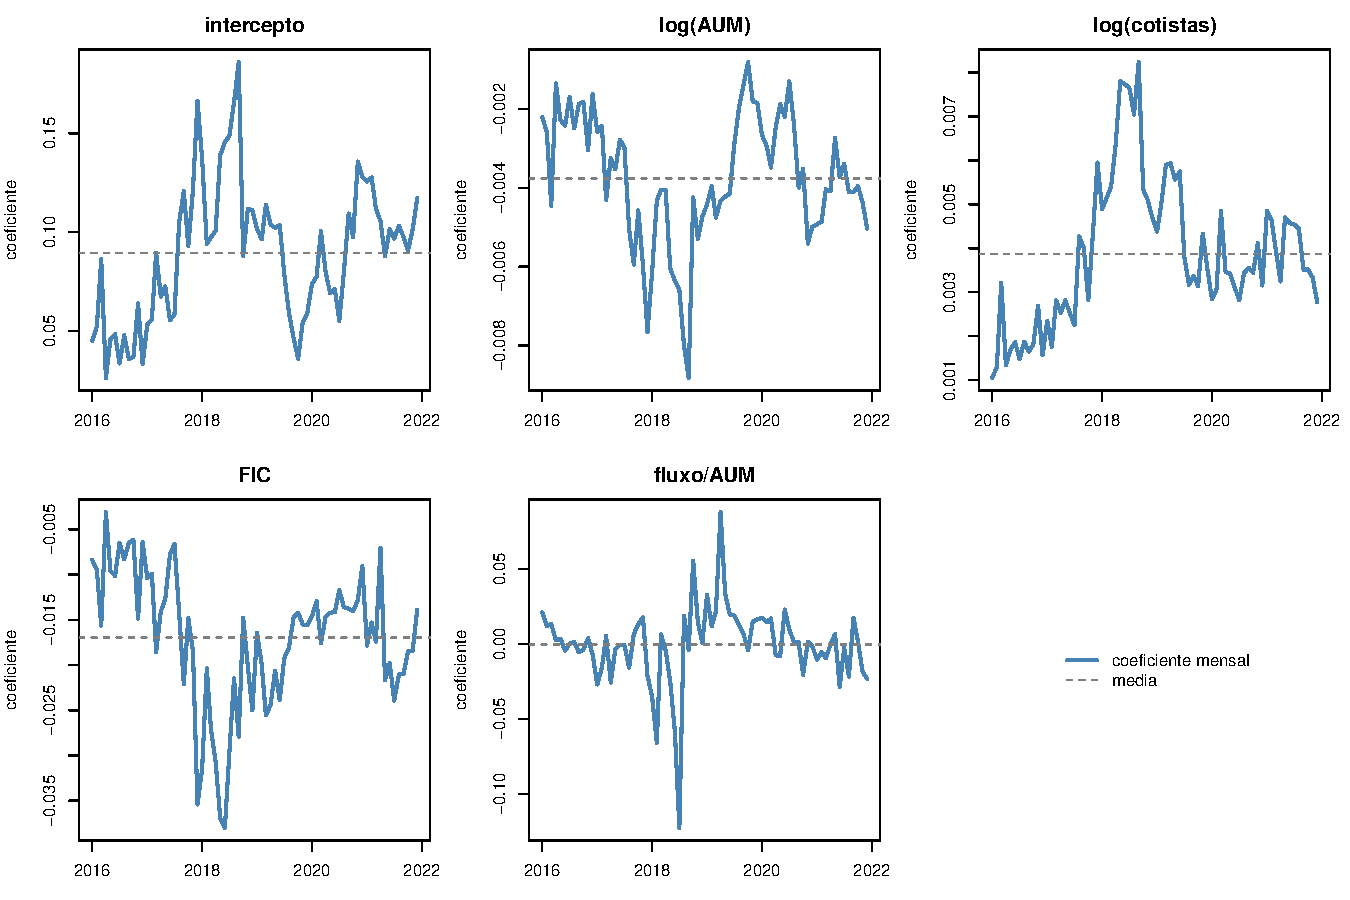
\includegraphics[width=0.80\textwidth]{fig_theta.pdf}
\caption{Coeficientes da regressão mês a mês, de 2016 a 2021. A linha tracejada marca a média
de cada série.}
\label{fig:theta}
\caption*{\footnotesize Fonte: elaboração própria.}
\end{figure}

\subsection{Previsão e a matriz de erros}

O resultado de previsão é o mais surpreendente e está na Tabela~\ref{tab:fc}. Avaliando fora
da amostra, nenhum modelo estrutural supera a previsão ingênua de repetir o último peso.
Acrescentar um nível próprio de cada fundo, por meio de um efeito fixo, ou prever os
coeficientes pelo filtro de Kalman, piora a previsão; modelar diretamente a variação do peso
apenas empata com a regra ingênua. O fato de a média histórica do próprio fundo prever pior
do que o último valor indica que o peso não reverte a uma média no nível do fundo, e sim que é
muito persistente, próximo de um passeio aleatório. Os erros do melhor modelo têm média
praticamente nula e formam uma série estacionária, propriedades que se desejava verificar.

\begin{table}[h]\centering\small
\caption{Erro de previsão fora da amostra, medido pela raiz do erro quadrático médio, nos
horizontes de um e de três meses.}
\label{tab:fc}
\begin{tabular}{@{}llrrrr@{}}
\toprule
Universo & Horizonte & Ingênua & Nível do fundo & Fator com Kalman & Variação do peso \\
\midrule
Todos os fundos      & 1 mês  & $0{,}0156$ & $0{,}0240$ & $0{,}0255$ & $0{,}0156$ \\
Todos os fundos      & 3 meses& $0{,}0207$ & $0{,}0262$ & $0{,}0273$ & $0{,}0210$ \\
Só fundos de ações   & 1 mês  & $0{,}0197$ & $0{,}0310$ & $0{,}0383$ & $0{,}0198$ \\
Só fundos de ações   & 3 meses& $0{,}0266$ & $0{,}0337$ & $0{,}0385$ & $0{,}0270$ \\
\bottomrule
\end{tabular}
\caption*{\footnotesize Fonte: elaboração própria.}
\end{table}

No horizonte de três meses a previsão ingênua piora, como era de esperar, e a distância para
os modelos estruturais diminui, mas ela ainda vence. Restringir a amostra apenas aos fundos
de ações não altera essa conclusão, apenas a torna mais nítida, pois nesses fundos as
posições em VALE3 são maiores e mais variáveis. A leitura prudente é a de que, no curto prazo,
a inércia do próprio fundo constitui um teto difícil de superar, e que o modelo de fator deve
ser visto, por ora, como ferramenta de compreensão, e não de previsão.

\subsection{As duas margens}

Por fim, separa-se a decisão de ter a ação da decisão de quanto carregar. A regressão
logística da probabilidade de o fundo ter VALE3 revela um padrão que se considera o mais
interessante do trabalho: as duas decisões têm sinais opostos, como sintetiza a
Tabela~\ref{tab:margens}. Fundos maiores e fundos de cotas são mais propensos a ter a ação,
mas, quando a têm, carregam um peso menor. Esse padrão é compatível com diversificação, no
sentido de que esses fundos espalham a carteira por muitas ações, incluindo VALE3, cada uma
com uma fatia pequena. A posse, por sua vez, é ainda mais persistente que o peso, e novamente
a previsão ingênua de repetir o estado anterior acerta muito mais do que o modelo com
características.

\begin{table}[h]\centering\small
\caption{Sinais opostos entre a decisão de ter a ação e a decisão de quanto carregar.}
\label{tab:margens}
\begin{tabular}{@{}lcc@{}}
\toprule
Característica & Ter ou não a ação & Quanto carregar \\
\midrule
Tamanho do fundo   & mais provável ter & peso menor \\
Fundo de cotas     & mais provável ter & peso menor \\
Número de cotistas & menos provável (efeito fraco) & peso maior \\
\bottomrule
\end{tabular}
\caption*{\footnotesize Fonte: elaboração própria.}
\end{table}

%==================== 5. CONCLUSÃO ====================
\section{Conclusão}

Este trabalho organizou, a partir das bases públicas da Comissão de Valores Mobiliários, um
painel mensal dos pesos da ação VALE3 nas carteiras dos fundos do grupo Itaú entre 2016 e
2021, e o utilizou para responder a duas perguntas. A primeira era quais características de um
fundo explicam o peso que ele atribui à ação. A segunda era se esse peso pode ser previsto de
um mês para o outro. A evidência reunida sugere respostas claras e, em parte, contrastantes.
O peso é bem explicado pela seção transversal, por tamanho do fundo, número de cotistas,
classificação de fundo de cotas e beta da ação, com sinais estáveis ao longo de todo o
período, e a decisão de ter a ação carrega sinais opostos aos da decisão de quanto carregar,
um padrão compatível com diversificação. Para previsão, contudo, nenhum dos modelos
estruturais testados supera a previsão ingênua de repetir o último peso, mesmo sob a
defasagem trimestral de divulgação das carteiras, de modo que o peso se comporta, no nível do
fundo, de forma muito persistente, próxima de um passeio aleatório.

A interpretação que se extrai é que o modelo de fator é, antes de tudo, uma ferramenta de
compreensão, capaz de revelar quais características importam para as posições, e não um modelo
de previsão de curto prazo, território em que a inércia do próprio fundo domina. Esse achado
deve ser lido à luz de algumas limitações. A análise restringe-se a uma única ação e a uma
única gestora, em um período específico, de modo que a generalização requer cautela. A
variável de captação sobre patrimônio apresenta caudas extremas em fundos de patrimônio
muito pequeno, ainda não tratadas. E o efeito mecânico do preço sobre o peso, separado apenas
de forma parcial do efeito de decisão ativa do gestor, merece tratamento mais cuidadoso.

As limitações apontam diretamente para a agenda futura, centrada no modelo de ajuste parcial
da carteira especificado na Seção 3. O passo seguinte é estimar a velocidade de ajuste pela
regressão regularizada da variação do peso sobre a distância ao peso desejado, verificar se
essa velocidade é estatisticamente diferente de zero e caracterizar a série de erros de
previsão sob a defasagem de divulgação. De forma complementar, pretende-se estender a análise
a outras ações e gestoras, aproveitando que o código construído é facilmente adaptável; tratar
as caudas extremas da variável de captação; decompor a parte do peso que muda apenas em razão
da variação do preço daquela que reflete decisão ativa; e modelar de forma mais formal a
margem extensiva por meio de um modelo em duas partes. Todo o código, os dados e o registro
das decisões metodológicas estão organizados no repositório do projeto, de modo a tornar os
resultados reprodutíveis.

%==================== REFERÊNCIAS ====================
\newpage
\addcontentsline{toc}{section}{Referências}
\section*{Referências}
\small
\begin{description}
\item Coval, Joshua and Erik Stafford. Asset fire sales (and purchases) in equity markets.
\emph{Journal of Financial Economics}, 86(2):479--512, 2007.
\item Fama, Eugene F. and James D. MacBeth. Risk, return, and equilibrium: empirical tests.
\emph{Journal of Political Economy}, 81(3):607--636, 1973.
\item Gabaix, Xavier and Ralph S. J. Koijen. In search of the origins of financial
fluctuations: the inelastic markets hypothesis. \emph{NBER Working Paper} 28967, 2021.
\item Harvey, Andrew C. \emph{Forecasting, Structural Time Series Models and the Kalman
Filter}. Cambridge University Press, Cambridge, 1989.
\item Hoerl, Arthur E. and Robert W. Kennard. Ridge regression: biased estimation for
nonorthogonal problems. \emph{Technometrics}, 12(1):55--67, 1970.
\item Koijen, Ralph S. J. and Motohiro Yogo. A demand system approach to asset pricing.
\emph{Journal of Political Economy}, 127(4):1475--1515, 2019.
\item Lou, Dong. A flow-based explanation for return predictability. \emph{Review of
Financial Studies}, 25(12):3457--3489, 2012.
\end{description}

\end{document}
